\chapter{Grundlagen}\label{grundlagen}

\section{Medizinische und messtechnische Grundlagen}

Die vorliegende Arbeit beschäftigt sich mit der Beurteilung der Signalqualität in ballistokardiographischen Signalen. Zum Verständnis der gemessenen Vorgänge und der Problematik in Bezug auf die Signalqualität und dessen Beurteilung ist grundlegendes medizinisches Wissen über die gemessenen Vorgänge und messtechnisches Verständnis nötig. Aufgrund dessen wird hier eine kurze Übersicht über die medizinischen Grundlagen gegeben.

	\subsection{Kardiorespiratorisches System}
	
	Das kardiorespiratorische System (zusammengesetzt aus \textit{kardìa}, deutsch 'Herz' und \textit{respiratio}, deutsch 'Atmung') setzt sich aus zwei Teilsystemen zusammen, dem kardiovaskulären und dem respiratorischen System, die zusammen die Versorgung der Organe mit sicherstellen.
	
	Das kardiovaskuläre System umfasst das Herz, die Arterien und die Venen. In einem Zyklus wird das sauerstoffreiche Blut von der linken Herzkammer durch die Arterien zu den Organen gepumpt, wo sich der Sauerstoff zur Versorgung dieser vom Blut löst. Die Venen transportieren das nun sauerstoffarme Blut in die rechte Herzkammer. Von dort wird es zur Lunge geführt, mit Sauerstoff angereichert und in die linke Herzkammer geleitet. Damit schließt sich der Zyklus. Die Herzfrequenz ist hierbei und relevanter messbarer Vitalparameter.
	
	Ein Herzschlag selbst besteht aus zwei Phasen: einer füllenden und einer auswerfenden Phase. Während der Diastole, der Erschlaffungs- und Bluteinströmungsphase, füllen sich die Herzkammern mit Blut. Diese Phase endet mit dem Schließen der Herzklappen und die Systole beginnt. Die Systole ist die Anspannungs- und Blutausströmungsphase: Die Herzklappen öffnen sich durch Kontraktion des Herzmuskels und das Blut kann ausströmen.
	
	Das respiratorische System umfasst die Lungen und den Lungenkreislauf. In einem Atemzyklus wird durch gezielte Muskelbewegungen Luft aus der Umgebung eingeatmet. Mit dem eingeatmeten Sauerstoff wird sauerstoffarmes Blut angereichert und anschließend die nun sauerstoffarme Luft ausgeatmet. Hier ist der Vitalparameter der Atemfrequenz messbar.

	\subsection{Übersicht Messtechniken}
			\begin{itemize}
				\item BKG oft mit anderen Messmethoden als Referenz
				\item EGK: Aufzeichnung elektrischer Aktivitäten des Herzmuskels (Spannungsänderung mit mehreren Elektroden) -> Herzfrequenz
				\item PPG: optisch, misst Menge des von Haut reflektierten/transmittierten Lichtes -> Änderung des Blutvolumens (Lichtmenge nimmt bei Durchlaufen einer Pulsmenge ab) -> Rückschluss auf Atmung und Herzschlag
				\item SKG: Vibrationen der Wand des Brustkorbs durch Herzschlag (oft mit BKG gemeinsam betrachtet)
			\end{itemize}


	\section{Ballistokardiographie}
	
	\subsection{Medizinischer und technischer Hintergrund}
	
	\begin{itemize}
		\item 
	\end{itemize}
	
	\subsection{Einsatzgebiet}
	\subsection{Signaleigenschaften}
	\subsection{Signalverarbeitung}

\section{Maschinelles Lernen}


% Beispiele Formeln
\[
\begin{gathered}
	y = +1, \text{ falls } \sum_{i=1}^{n} w_i \cdot x_i > b \\
	y = -1, \text{ falls } \sum_{i=1}^{n} w_i \cdot x_i < b
\end{gathered}
\]

\[
qSQI = \begin{cases}
	\text{excellent (E)} & \text{wenn alle 4 } SQI_i \geq 0,9\\
	\text{acceptable (A)} & \begin{cases}
		& \text{wenn 3 der 4 } SQI_i \geq 0,9 \text{ oder}\\
		& \text{wenn alle 4 } SQI_i \geq 0,7 \text{ oder}\\
		& \text{wenn median}(SQI_1, SQI_2, SQI_3) \geq 0,8\\&\text{ }\text{	und } SQI_1 \geq 0,5 \text{ und } SQI_4 \geq 0,7
		\end{cases}\\
	\text{untrustworthy (U)} & \text{sonst}\\
\end{cases}
\]

% Beispiel figure

\begin{figure}[H]
	\centering
		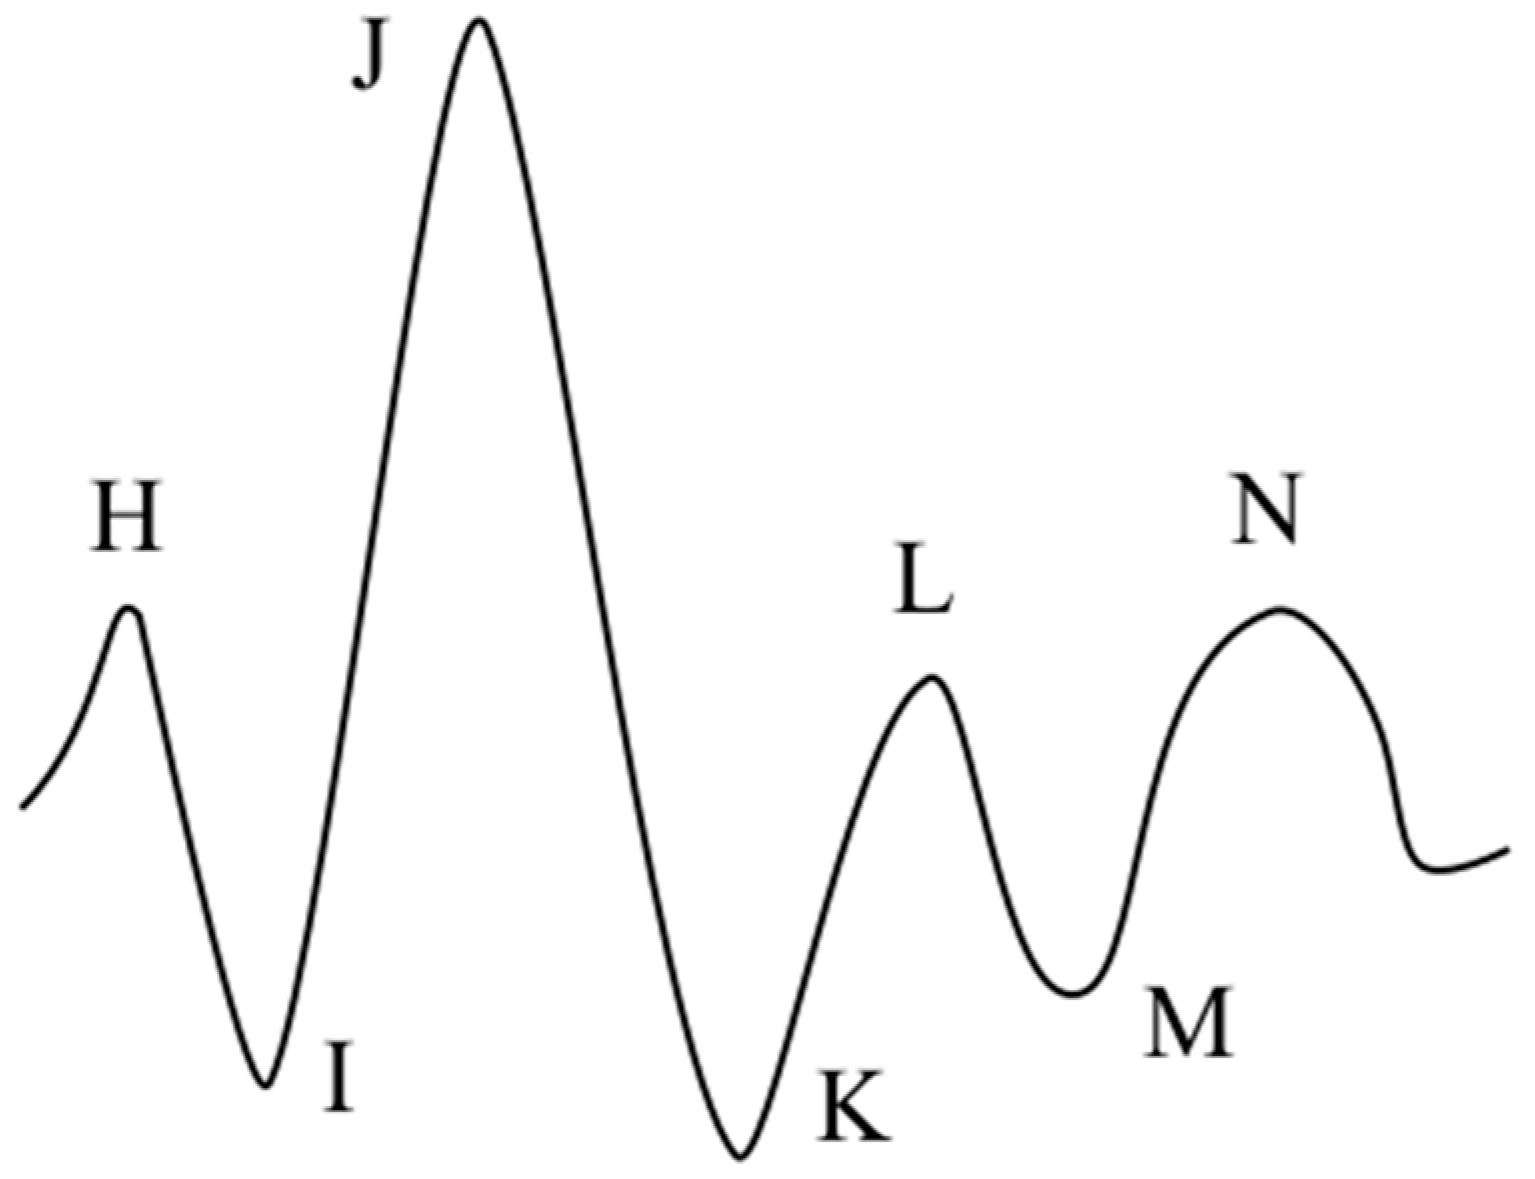
\includegraphics[width=0.7\textwidth]{pic/bcgWaveform.png}
	\caption[Beispiel eines typischen \ac{BKG}-Signals mit Nomenklatur]{Beispiel eines typischen \ac{BKG}-Signals mit Nomenklatur\protect\footnotemark}
	\label{fig:bcgwaveform}
\end{figure}
\footnotetext{Entnommen aus \cite{Albukhari2019} nach \cite{Starr1939}.}
